
In this section, the obtained results from a Gaussian mixture training are reviewed. Two out of three frameworks are tested in this model.

\section{InferPy}

Firstly, the model cannot be directly modeled using \texttt{InferPy} due to the fact that \texttt{TensorFlow} \texttt{-Probability} name them as \texttt{NOT\_REPARAMETERIZED}, which in its documentation says ``If NOT\_REPARAMETERIZED, then samples from the distribution are not fully reparameterized, and straight-through gradients are either partially unsupported or are not supported at all''. Unsuccessful attempts have being made using \texttt{MixtureGaussian} distribution available in \texttt{InferPy}.


\section{BayesPy}

The \texttt{BayesPy} model can be easily created using the syntax explained before, the model parameters are initialized as
\begin{itemize}
  \item The means variable $\mu$ follows a centered normal distribution:
  $$\mu_k \sim \mathcal{N}_{data\_dim}(0,I).$$
  \item The precision variables $\Lambda$ follow a Wishart distribution with parameters:
  $$\Lambda_k \sim \mathcal{W}_{data\_dim}(data\_dim, I).$$
  \item The weights concentration variable follows a Dirichlet with parameter:
  $$ \pi \sim \text{Symmetric-Dirichlet}\Big(\frac{1}{n\_classes}\Big).$$
\end{itemize}

Which is coded as the following.
\begin{minted}{python}
    Lambda = nodes.Wishart(dim, np.identity(dim), plates=(n_components,))
    mu = nodes.Gaussian(np.zeros(dim), 0.01 * np.identity(dim), plates=(n_components,))
    pi = nodes.Dirichlet(0.01 * np.ones(n_components))
    z = nodes.Categorical(pi, plates=(n_samples,))
    x = nodes.Mixture(z, nodes.Gaussian, mu, Lambda)
\end{minted}

We start using a testing 2D database made of 4 components:
$$
\mathcal{N}\Bigg(\begin{pmatrix} 0 \\ 0 \end{pmatrix}, \begin{pmatrix} 0.2 & 0 \\ 0 & 0.2\end{pmatrix} \Bigg) \quad \mathcal{N}\Bigg(\begin{pmatrix} 1 \\ 1 \end{pmatrix}, \begin{pmatrix} 0.1 & 0 \\ 0 & 0.2\end{pmatrix} \Bigg)
$$
$$
\mathcal{N}\Bigg(\begin{pmatrix} 3 \\ 0 \end{pmatrix}, \begin{pmatrix} 0.2 & 0.1 \\ 0.1 & 0.2\end{pmatrix} \Bigg) \quad \mathcal{N}\Bigg(\begin{pmatrix} -2 \\ 0 \end{pmatrix}, \begin{pmatrix} 0.2 & 0 \\ 0 & 0.2\end{pmatrix} \Bigg)
$$
With concentrations \([0.29\ 0.29\ 0.24\ 0.18]\) respectively. After the model training, the results can be plotted using \texttt{BayesPy} \texttt{bbplt} function (Figure~\ref{fig:mix_test_bayespy}). In this plotting, both the dataset and the learned distributions can be seen.

\begin{figure}[h!]
    \centering
    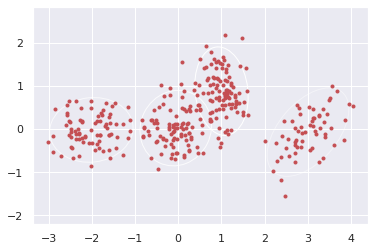
\includegraphics[width=0.7\textwidth]{tex/images/mixture_testing_bayespy.png}
    \caption{Testing database plot with learned distributions.}\label{fig:mix_test_bayespy}
\end{figure}

We might inspect the posterior of any variable, for example, the posterior for \(\bmu\) is:

$$
\mathcal{N}\Bigg(\begin{pmatrix} -0.05 \\ 0.02 \end{pmatrix}, \begin{pmatrix} 0.017 & 0.00012 \\ 0.00012 & 0.019\end{pmatrix} \Bigg)
\quad
\mathcal{N}\Bigg(\begin{pmatrix} 1.002 \\ 0.8991 \end{pmatrix}, \begin{pmatrix} 0.0001 & -0.0002 \\ -0.0002 & 0.002 \end{pmatrix} \Bigg)
$$
$$
\mathcal{N}\Bigg(\begin{pmatrix} 3.0065 \\ -0.0689 \end{pmatrix}, \begin{pmatrix} 0.0037 & 0.0021 \\ 0.0021 & 0.0043 \end{pmatrix} \Bigg)
\quad
\mathcal{N}\Bigg(\begin{pmatrix} -2.0117 \\ -0.01762 \end{pmatrix}, \begin{pmatrix} 0.0029 & 0.0001 \\ 0.0001 & 0.0025 \end{pmatrix} \Bigg)
$$

which shows how the model has correctly learn the mean values with a relatively low deviation.

Due to the high number of attributes (784) in \texttt{Mnist} database, \texttt{BayesPy} is not able to handle the VMP algorithm with a great number of samples (it attempts to locate a matrix with shape \((n\_samples,\ n\_components,\ 784,\ 784)\)). For this reason, \texttt{Breast Cancer} is used.

The model is created with the same number of components as different classes (2) in an attempt to learn one Gaussian distribution for each class. After the inference task, \texttt{BayesPy} does not provide any way of plotting high dimensional results. On the other hand, using \texttt{x.random()} we are able to generate posterior samples.

\section{Scikit-Learn}

In this occasion we are using 1000 samples from classes \([1,4,7]\) from \texttt{Mnist}. The model is created as explained in the previous section using the same prior values we used in \texttt{BayesPy}.

One of the parameters that can be easily studied is the weight of each component:
\begin{minted}{python}
  print(gm.weights_)
\end{minted}
Which resulted in \([0.26806527\  0.38994339\ 0.34199134]\). The posterior predictive can be used to test the models accuracy
\begin{minted}{python}
  print(sum(gm.predict(X) == y)/n_samples)
\end{minted}
Which shows a precision of 0.339.
